\section{Results}\label{sec:results}
All numbers were measured on data the models never trained on (Section~\ref{sec:setup}).

\subsection{RQ1: naming poses on held-out photos}\label{sec:rq1}
Table~\ref{tab:frame} and Fig.~\ref{fig:charts}a compare the cascade, its components and five standard classifiers on the 1{,}685 held-out public photos and on the wild set. The cascade names the pose on 78.9\% of the photos with a 20.8\% false-alarm rate and seven poses at recall and precision $\ge0.70$ (chair, corpse, downward dog, tree, triangle, upward dog, Warrior~II), against 36.9\%, 78.3\% and none for the rule engine alone. The veto is what matters: the namer alone recalls poses well but accepts nearly everything (81.5\% false alarms), and the gate model alone is accurate but passes fewer poses (three). The decision rule was chosen on a validation half of the photos (79.3\%, 20.1\%, three poses) and held on the untouched half (78.6\%, 21.6\%, four poses).
\begin{table}[t]
\centering\footnotesize\setlength{\tabcolsep}{3.5pt}
\caption{Frame-level naming on two held-out sets (bold: best in column). Public: 1{,}685 photos from the training sources, 1{,}037 of other poses. Wild: 103 Commons photos from another source, out-of-fold. $^\dagger$single earlier run.}\label{tab:frame}
\begin{tabular}{@{}lrrrr@{}}
\toprule
 & \multicolumn{3}{c}{Public held-out} & Wild \\
Method & Overall & False alarm & Poses pass & Overall \\ \midrule
Rule engine only & 36.9\% & 78.3\% & 0 & 37.9\% \\
Logistic regression$^\dagger$ & 29.7\% & 95.8\% & 1 & -- \\
$k$-NN & 58.6\% & 55.7\% & 1 & 50.5\% \\
SVM (RBF) & 58.4\% & 56.2\% & 3 & 52.4\% \\
Plain MLP & 80.9\% & 19.1\% & 3 & 47.6\% \\
Random forest & \textbf{85.3\%} & \textbf{9.8\%} & \textbf{7} & 35.0\% \\
Namer alone & 42.9\% & 81.5\% & 1 & \textbf{60.2\%} \\
Gate model alone & 79.6\% & 22.6\% & 3 & 49.5\% \\
Average of namer and gate & 65.2\% & 47.7\% & 5 & -- \\
Veto lifted when rules agree & 65.9\% & 42.3\% & 5 & -- \\
Cascade (ours) & 78.9\% & 20.8\% & \textbf{7} & 55.3\% \\ \bottomrule
\end{tabular}
\end{table}

\runin{A result against our design.} A random forest on the same 15 angles beats the cascade on photos from the training sources (85.3\% against 78.9\%, 9.8\% against 20.8\% false alarms). We checked whether this is memorisation of near-duplicates: only 0.3\% of the held-out photos lie within 0.05 (standardised angle units) of a training photo, and the forest's lead holds in every quartile of distance to the nearest training photo, including the farthest (84.6\% against 77.0\%). But on the wild set the ranking reverses: the forest is the weakest learned method (35.0\%), 13--25 points below every other learned method, and the cascade (55.3\%) is within five points of the best (60.2\%). A plain MLP matches the residual gate on public photos (80.9\% against 79.6\%), so the residual trunk is not what buys accuracy; what the 3-head design adds is the form and deviation outputs from one small forward pass. We conclude that no single classifier is best on both sources, that the cascade is within seven points of the best on each and keeps false alarms near 21\%, and that a tree--network ensemble is the obvious next experiment.

\runin{Why random splits mislead.} A model of the same architecture trained and validated on a random split, as is common, reached 91.5\% validation accuracy but named only 26.8\% of 422 unseen photos correctly, and an ST-GCN validated the same way reached 82.6\% validation accuracy but only 11.6\% macro recall on held-out videos.

\begin{figure*}[t]
\centering
\begin{subfigure}[t]{0.32\textwidth}\centering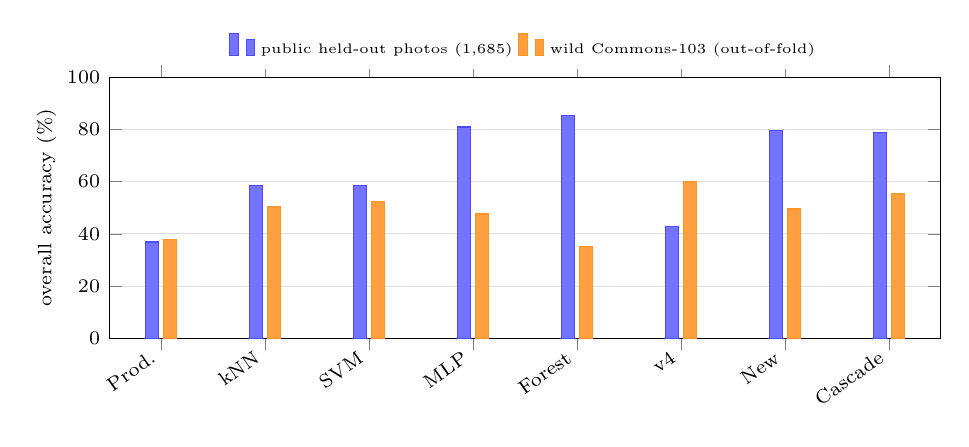
\begin{tikzpicture}
\begin{axis}[ybar,bar width=4.6pt,width=\columnwidth,height=4.9cm,ymin=0,ymax=100,ylabel={overall accuracy (\%)},ylabel style={font=\scriptsize,yshift=-3pt},
  symbolic x coords={Prod.,kNN,SVM,MLP,Forest,v4,New,Cascade},xtick=data,x tick label style={font=\scriptsize,rotate=35,anchor=east},y tick label style={font=\scriptsize},
  legend style={font=\tiny,at={(0.5,1.03)},anchor=south,legend columns=2,draw=none},enlarge x limits=0.07,ymajorgrids,grid style={gray!25}]
\addplot[fill=blue!55,draw=blue!70] coordinates {(Prod.,36.9)(kNN,58.6)(SVM,58.4)(MLP,80.9)(Forest,85.3)(v4,42.9)(New,79.6)(Cascade,78.9)};
\addplot[fill=orange!75,draw=orange!85] coordinates {(Prod.,37.9)(kNN,50.5)(SVM,52.4)(MLP,47.6)(Forest,35.0)(v4,60.2)(New,49.5)(Cascade,55.3)};
\legend{public held-out photos (1{,}685),wild Commons-103 (out-of-fold)}
\end{axis}
\end{tikzpicture}
\caption{Frame-level methods, public vs.\ wild}\end{subfigure}\hfill
\begin{subfigure}[t]{0.32\textwidth}\centering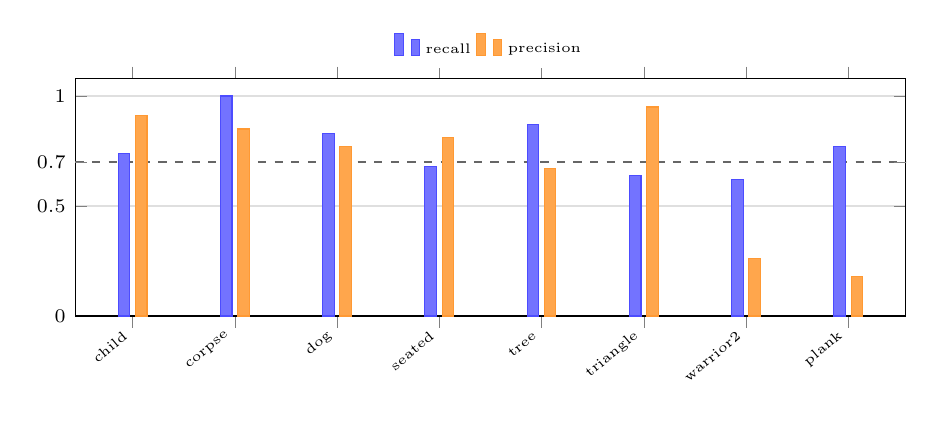
\begin{tikzpicture}
\begin{axis}[ybar,bar width=4.2pt,width=\linewidth,height=4.6cm,ymin=0,ymax=1.08,
  symbolic x coords={child,corpse,dog,seated,tree,triangle,warrior2,plank},xtick=data,x tick label style={font=\tiny,rotate=40,anchor=east},y tick label style={font=\scriptsize},
  legend style={font=\tiny,at={(0.5,1.04)},anchor=south,legend columns=2,draw=none},enlarge x limits=0.08,ymajorgrids,grid style={gray!25},
  extra y ticks={0.7},extra y tick style={grid=major,grid style={dashed,black!60},tick label style={font=\tiny}}]
\addplot[fill=blue!55,draw=blue!70] coordinates {(child,0.74)(corpse,1.00)(dog,0.83)(seated,0.68)(tree,0.87)(triangle,0.64)(warrior2,0.62)(plank,0.77)};
\addplot[fill=orange!70,draw=orange!80] coordinates {(child,0.91)(corpse,0.85)(dog,0.77)(seated,0.81)(tree,0.67)(triangle,0.95)(warrior2,0.26)(plank,0.18)};
\legend{recall,precision}
\end{axis}
\end{tikzpicture}
\caption{Flow check, held-out videos, per pose}\end{subfigure}\hfill
\begin{subfigure}[t]{0.32\textwidth}\centering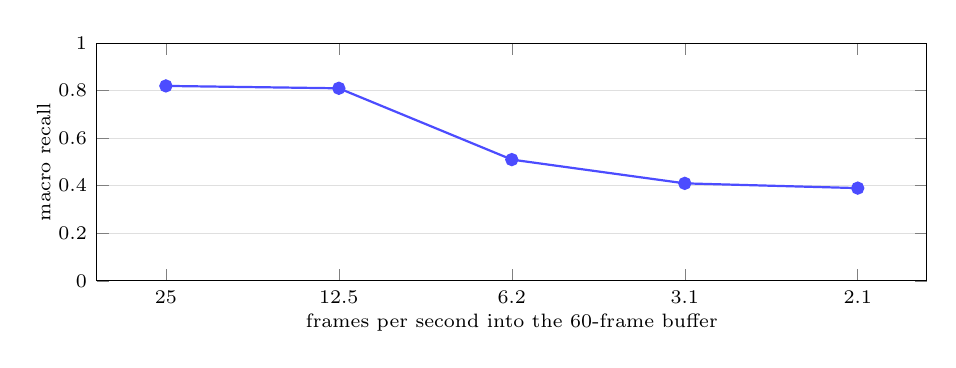
\begin{tikzpicture}
\begin{axis}[width=\linewidth,height=4.6cm,ymin=0,ymax=1,symbolic x coords={25,12.5,6.2,3.1,2.1},xtick=data,x tick label style={font=\scriptsize},y tick label style={font=\scriptsize},
  xlabel={frames per second into the 60-frame buffer},xlabel style={font=\scriptsize,yshift=3pt},ylabel={macro recall},ylabel style={font=\scriptsize,yshift=-4pt},
  ymajorgrids,grid style={gray!25},enlarge x limits=0.1]
\addplot[blue!70,mark=*,thick] coordinates {(25,0.82)(12.5,0.81)(6.2,0.51)(3.1,0.41)(2.1,0.39)};
\end{axis}
\end{tikzpicture}
\caption{Flow check vs.\ input rate}\end{subfigure}
\caption{(a)~Overall accuracy of the methods of Table~\ref{tab:frame} on the two held-out sets (Prod.: rule engine only; New: gate model alone). (b)~Per-pose recall and precision of the temporal network on videos it never trained on (dashed: 0.70 bar; Warrior~II and plank have few windows). (c)~Macro recall when the 60-frame buffer is filled at different rates.}
\label{fig:charts}
\end{figure*}

\subsection{RQ2: the skeleton-graph temporal network}\label{sec:rq2}
On three folds split by video, the network reaches 82.2\% overall; because 60\% of the 8{,}002 windows are transition/unknown this flatters it, so we also report 78.0\% macro recall over the nine classes (76.9\% over the eight poses). Three poses clear the bar: child's pose (recall/precision $.74/.91$), corpse ($1.00/.85$) and downward dog ($.83/.77$); seated easy, tree and triangle are within about 0.07 of it (Fig.~\ref{fig:charts}b). The network is conservative: its misses go to transition/unknown, not to another pose. Warrior~II and plank fail on precision ($.26$, $.18$): 158 transition windows are called Warrior~II, and plank has only 30 windows. A less conservative threshold chosen without leakage (an offset on the transition logit, picked on two folds and applied to the third) raises the passing poses to four with 81.9\% overall; no offset reaches six. At the production confidence the network answers on 60.8\% of true-pose windows with 86.8\% precision.

\runin{Input rate.} Re-scoring the same videos while subsampling every $k$-th frame shows that the network needs windows at the rate it was trained on: macro recall is 0.82 at 25\,fps and 0.81 at 12.5\,fps, then falls to 0.51, 0.41 and 0.39 at 6.2, 3.1 and 2.1\,fps (Fig.~\ref{fig:charts}c). Feeding it one frame per server round trip would therefore silently destroy its accuracy, which is why the browser buffers every camera frame and resamples to 25\,fps.
\runin{Is the skeleton graph needed?} Table~\ref{tab:seq} trains six sequence models under one recipe and scores them on the same held-out folds. Three findings. First, the skeleton graph helps only a little over the same network without it (macro recall 86.4\% against 84.8\%, while overall accuracy is 76.0\% against 77.1\%); differences of one or two points are smaller than the seed-to-seed variation we did not measure. Second, simpler models match or exceed the ST-GCN: the LSTM, BiLSTM and temporal CNN reach 89.5--89.7\% macro recall, and an 86\,k-parameter MLP on the window's mean and standard deviation, which has no temporal modelling at all, is best (94.4\%). Held-pose recognition is therefore largely a static-shape problem, and we do not claim that the graph is necessary for it. Third, every model shares one weakness: Warrior~II (precision 0.24--0.30) and plank (0.10--0.40, 30 windows) are over-called because transition windows are labelled as poses, while transition/unknown itself has high precision (0.91--0.96). An ST-GCN fold takes about 290\,s to train on a T4, against 6--15\,s for the others. The absolute numbers differ from the production figures above (macro recall 86.4\% against 78.0\%, overall 76.0\% against 82.2\%) because this recipe uses fewer windows, fixed epochs and class weights, which trade overall accuracy for recall; the comparison within the table is what matters. We keep the ST-GCN as a second opinion and as the basis for flow scores (smoothness, balance, momentum) that static statistics cannot provide, but the evidence for it today is parity, not superiority.
\runin{Does the network model movement?} Held-pose recognition is a static task, and the network is meant to capture how the body moves between poses, so we also tried to test movement. Our labels do not allow a named-transition benchmark: of the 568 consecutive hold pairs in the 24 videos, 205 are between different poses, and within 500 frames (70 transitions in 33 directional pairs) no pair occurs in three or more videos. We therefore built a rule-defined movement task: a window is a transition when its net angle change exceeds 15\textdegree/s and is named by the dominant pose of its first and last third, otherwise a hold or unrecognised, which gives 19 classes after dropping those with fewer than 100 windows or fewer than three videos (16 holds, generic transition, unrecognised, and one named transition, cobra pose to downward dog). The labels are defined by rules, so the task measures whether a model recovers rule-defined flow from the raw skeleton, not agreement with an annotator. The last column of Table~\ref{tab:seq} shows the same ordering as for held poses: the window-statistics MLP is best (58.6\% macro recall), the ST-GCN last (47.7\%), and removing the skeleton graph changes nothing measurable (48.4\%). A time-reversal test (every moving window shown forward and reversed, chance 50\%) is at chance for every model (49.9--51.1\%), so under this recipe no model, including the ST-GCN, is shown to use the direction of time; the test is uninformative, not evidence either way. We therefore make no claim that the network models movement; labelled transition data is the missing ingredient (Section~\ref{sec:discussion}).

\runin{Does 3D matter?} The sequence models are the only models fed the depth coordinate $z$ (the per-frame MLPs use angles computed with $z{=}0$). Retraining the same models with $z$ set to zero (Table~\ref{tab:z}) lowers every model on both tasks: by 20 points (temporal CNN) and 35 points (MLP) on held poses, while the ST-GCN collapses from 88.7\% to 28.6\% macro recall, most windows then falling to the generic transition class; on the movement task the loss is 4 to 12 points. The depth coordinate is therefore the largest effect we measured, larger than the choice among sequence models, and the sequence input is how three-dimensional information enters the system. Caveats: $z$ is MediaPipe's monocular relative depth, not measured depth; the figures are for 24 videos and one seed; and the $z$ a phone camera produces live may differ from that of the training videos.

\begin{table}[t]
\centering\footnotesize\setlength{\tabcolsep}{3pt}
\caption{Effect of the depth coordinate: macro recall of the same models trained with the full $(x,y,z)$ skeleton and with $z$ set to zero (bold: best in column). Held poses: nine classes on the cueT2 video folds; Movement: the 19-class rule-defined task. At most 3{,}000 training windows per class and one seed, so the full-skeleton held-pose values differ slightly from Table~\ref{tab:seq}.}\label{tab:z}
\begin{tabular}{@{}lrrrr@{}}
\toprule
 & \multicolumn{2}{c}{Held poses} & \multicolumn{2}{c}{Movement} \\ \cmidrule(lr){2-3}\cmidrule(lr){4-5}
Model & $x,y,z$ & $z{=}0$ & $x,y,z$ & $z{=}0$ \\ \midrule
MLP on window mean/std & \textbf{94.2\%} & 59.3\% & \textbf{59.5\%} & 46.3\% \\
Temporal CNN & 90.5\% & \textbf{70.1\%} & 56.2\% & \textbf{52.1\%} \\
ST-GCN & 88.7\% & 28.6\% & 47.5\% & 35.9\% \\ \bottomrule
\end{tabular}
\end{table}

\begin{table}[t]
\centering\footnotesize\setlength{\tabcolsep}{3pt}
\caption{Sequence models under one recipe on the held-out video folds (bold: best in column; for parameters, fewest). MR9: macro recall over the nine classes; MR8: over the eight poses; Pass: poses at recall and precision $\ge0.70$; Flow: macro recall over the 19 classes of the rule-defined movement task (24 videos, 3 folds by video).}\label{tab:seq}
\begin{tabular}{@{}lrrrrrr@{}}
\toprule
Model & Params & Overall & MR9 & MR8 & Pass & Flow \\ \midrule
LSTM (2 layers) & 0.25\,M & 83.0\% & 89.5\% & 91.0\% & 4 & 53.1\% \\
BiLSTM + attention & 0.50\,M & \textbf{87.1\%} & 89.6\% & 90.1\% & \textbf{5} & 56.8\% \\
Temporal CNN & 1.00\,M & 81.5\% & 89.7\% & 91.4\% & 4 & 55.6\% \\
MLP on window mean/std & \textbf{0.09\,M} & 85.3\% & \textbf{94.4\%} & \textbf{96.4\%} & \textbf{5} & \textbf{58.6\%} \\
ST-GCN, no skeleton graph & 0.89\,M & 77.1\% & 84.8\% & 86.4\% & 4 & 48.4\% \\
ST-GCN (ours) & 0.89\,M & 76.0\% & 86.4\% & 88.6\% & 4 & 47.7\% \\ \bottomrule
\end{tabular}
\end{table}


\subsection{RQ3: hidden joints}\label{sec:rq3}
We hid one limb with a grey box on 70 real yoga frames in four poses (141 cases) and recovered the hidden joints in three ways, with MediaPipe on the clean frame as the reference. Without recovery the median joint-angle error is $17.9^\circ$. Table~\ref{tab:cliff} compares left--right mirroring with CLIFF \cite{li2022cliff}. Neither dominates: mirroring is better where the body is symmetric (arms, mountain, seated) and has the lowest median landmark error overall, CLIFF is better for legs, for both feet hidden and for the asymmetric Tree pose, and its median angle error is $5.8^\circ$ against $8.6^\circ$. But CLIFF costs 164\,ms per image on two CPU threads (18.7\,ms on a T4 GPU) and, decisively, needs the image, which the app never sends. We therefore keep the abstain policy: a hidden joint is not scored, and the interface says which joints are not being checked. Caveats: 141 cases from 70 frames, one asymmetric pose, a synthetic occluder and MediaPipe, not motion capture, as the reference.
\begin{table}[t]
\centering\footnotesize
\caption{Recovering hidden joints: median joint-angle error in degrees (bold: lower).}\label{tab:cliff}
\begin{tabular}{@{}lrr@{}}
\toprule
Subset ($n$) & Mirror & CLIFF \\ \midrule
All (141) & $8.6$ & $\mathbf{5.8}$ \\
Symmetric stances (117) & $\mathbf{5.2}$ & $6.1$ \\
Tree, asymmetric (24) & $20.1$ & $\mathbf{4.8}$ \\
Left leg hidden (47) & $16.2$ & $\mathbf{6.2}$ \\
Right arm hidden (47) & $\mathbf{4.9}$ & $15.1$ \\
Both feet hidden (47) & $6.1$ & $\mathbf{4.7}$ \\ \bottomrule
\end{tabular}
\end{table}

\subsection{RQ4: form score, personal profile and efficiency}\label{sec:form}
\runin{Form score.} No labelled good-versus-bad-form data exist for these poses, so we use a property test: on 648 held-out in-vocabulary photos, five trials each, one joint is broken by $45^\circ$. The gate's form score is high on good form (0.81) and drops in 85.0\% of trials, while the deviation head's top-ranked joint is the broken one in only 12.4\% of trials (chance 6.7\%), which is why joint-level cues come from the angle bands. On the deployed endpoint with real MediaPipe angles from eight instructor clips the mean score is 0.94 while held, 0.25 with the left knee broken and 0.92 with the left elbow broken: the score collapses for leg errors and is nearly blind to arm errors (these clips are in the gate's training data, so this checks the deployed path, not generalisation).

\runin{Personal profile.} We tested the mechanism on the deployed server with a hand-built skeleton whose two hip deviations were $56^\circ$ from their bands (universal score 0.924). Without a profile the response carries no personal score; a profile not containing the current angles leaves it at 0.924; one containing the left hip's angle zeroes that deviation (0.962); both hips give 1.000; the universal score never changes. A profile spanning $0^\circ$--$180^\circ$ for every joint also gives 1.000, which shows how much a poor profile could forgive; the profile has not been validated with users.

\runin{Efficiency and hardware.} Table~\ref{tab:eff} lists model size and latency. Server compute is 7--9\,ms per frame (p95 8--11\,ms) with 324\,MB peak memory for all three networks, but the round trip from India is 0.97\,s at the median because it is dominated by the network; the interface therefore draws the skeleton locally (about 22 updates/s on the phone) and refreshes score and cue about every 1.5\,s, with the flow check and speech at about 10\,s. On the phone the pose engine scales with the number of Web Workers (7.3, 19 and 24 results/s for one, two and three).
\begin{table}[t]
\centering\footnotesize
\caption{Model size and measured latency.}\label{tab:eff}
\begin{tabular}{@{}lr@{}}
\toprule
Item & Measured \\ \midrule
Pose MLP (two models, cascade) & 0.36\,M parameters each \\
ST-GCN flow check & 0.89\,M parameters \\
Server compute per frame, median (p95) & 7--9\,ms (8--11\,ms) \\
Peak server memory, three networks & 324\,MB \\
Round trip, median (p95), $n{=}32$ & 967\,ms (1{,}266\,ms) \\
Phone engine, 1 / 2 / 3 workers & 7.3 / 19 / 24 results/s \\
Mesh recovery (CLIFF), 2 CPU threads & 164\,ms per image \\ \bottomrule
\end{tabular}
\end{table}

\subsection{End-to-end validation on a phone}\label{sec:phone}
We ran the real app on the phone through its CPU engine, with a Wikimedia photo standing in for the camera, and logged every answer of the live server; a photo counts if the most frequent of three answers is the expected pose, and a pose passes at 50\% or more of its photos (Table~\ref{tab:phone}). Eight of eleven poses pass; the six poses of the held-out benchmark that were tested all pass, while mountain, cobra and child's pose do not. These are still photos with labels taken from file titles, and some may have been seen in training, so the test validates the on-phone path (engine, landmarks, server, label), not generalisation. Fig.~\ref{fig:ui} shows the interface in three languages, both themes and both modes, and Fig.~\ref{fig:proof} shows hidden-joint handling, the calibration screens and a failure case.
\begin{table}[t]
\centering\footnotesize
\caption{On-phone photo test (photos correct / tested; a pose passes at 50\% or more). Two photos had no person found.}\label{tab:phone}
\begin{tabular}{@{}lc@{\hspace{8pt}}lc@{\hspace{8pt}}lc@{}}
\toprule
Pose & Correct & Pose & Correct & Pose & Correct \\ \midrule
Tree & 6/6 & Triangle & 5/5 & Warrior II & 3/3 \\
Downward dog & 4/4 & Seated easy & 4/5 & Plank & 3/4 \\
Chair & 3/5 & Corpse & 2/4 & Child's pose & 1/3 \\
Cobra & 1/5 & Mountain & 0/5 & & \\ \bottomrule
\end{tabular}
\end{table}

\begin{figure*}[t]
\centering
\begin{subfigure}[t]{0.165\textwidth}\centering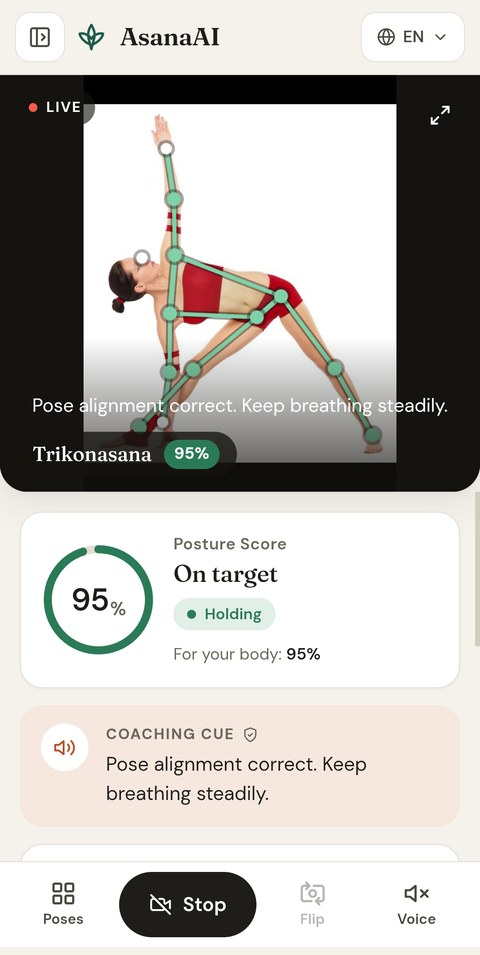
\includegraphics[width=\linewidth]{figures/ui_triangle_en.jpg}\caption{English, light}\end{subfigure}\hfill
\begin{subfigure}[t]{0.165\textwidth}\centering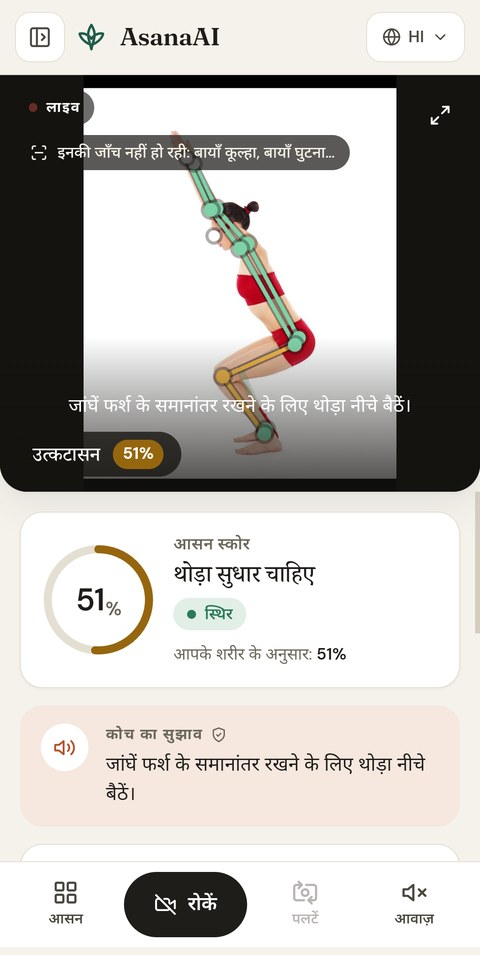
\includegraphics[width=\linewidth]{figures/ui_chair_hi.jpg}\caption{Hindi, 51\% form}\end{subfigure}\hfill
\begin{subfigure}[t]{0.165\textwidth}\centering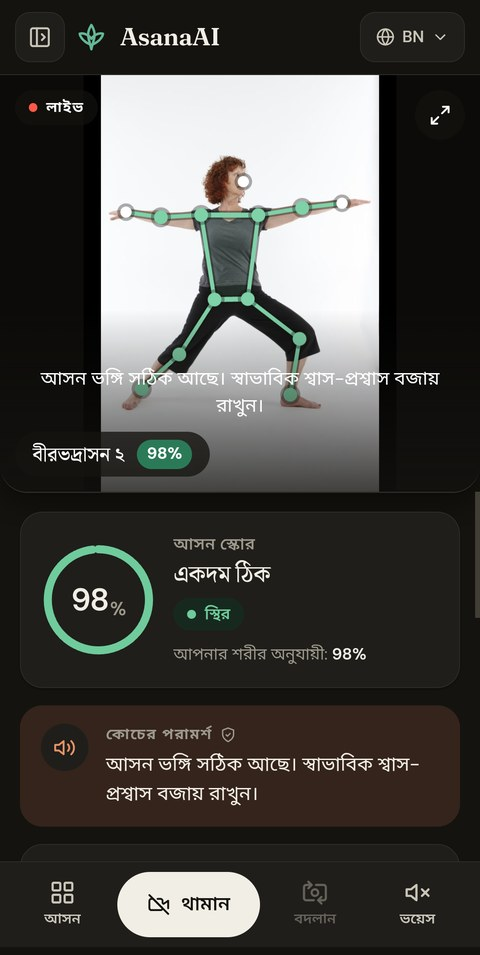
\includegraphics[width=\linewidth]{figures/ui_warrior_bn_dark.jpg}\caption{Bengali, dark}\end{subfigure}\hfill
\begin{subfigure}[t]{0.165\textwidth}\centering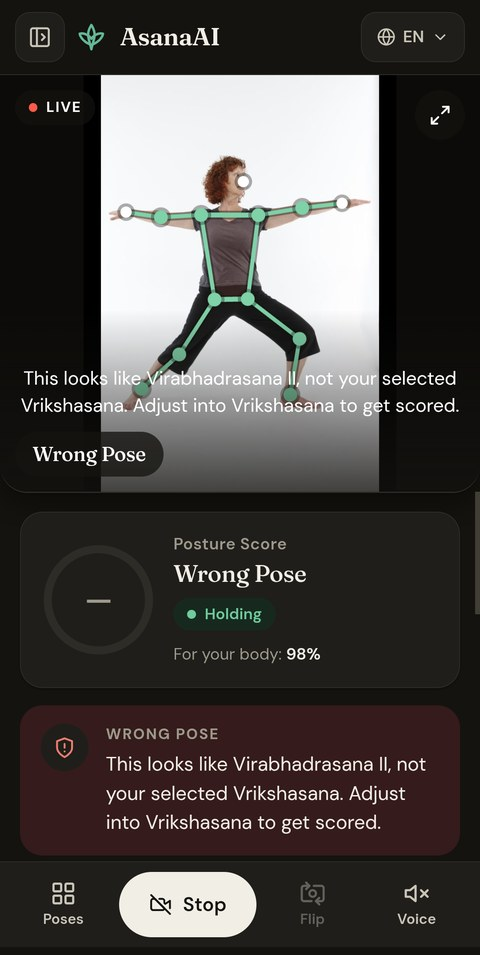
\includegraphics[width=\linewidth]{figures/ui_guided_wrong.jpg}\caption{Guided: wrong pose}\end{subfigure}\hfill
\begin{subfigure}[t]{0.165\textwidth}\centering
\includegraphics[width=\linewidth]{figures/landing_light.jpg}\caption{Landing page}\end{subfigure}
\caption{The deployed interface on a POCO M7 Pro, a credited Wikimedia photograph standing in for the camera (no live person): (a)~Trikonasana, 95\%; (b)~Utkatasana with the Hindi cue, 51\% in amber and a chip naming the joints not checked; (c)~Virabhadrasana~II in Bengali; (d)~guided mode with Vrikshasana selected while a Warrior~II photo is shown: the score is withheld and the app names the pose it sees; (e)~the public landing page. Photos by Kennguru (a, b; CC BY 3.0) and lululemon athletica (c, d; CC BY 2.0), via Wikimedia Commons.}
\label{fig:ui}
\end{figure*}
\begin{figure*}[t]
\centering
\begin{subfigure}[t]{0.19\textwidth}\centering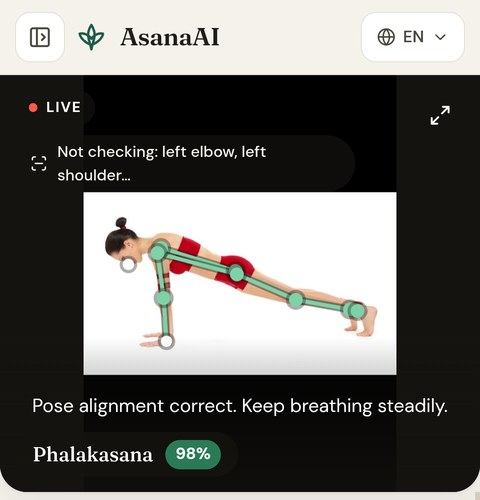
\includegraphics[width=\linewidth]{figures/oc_plank_hidden.jpg}\caption{Hidden joints not judged}\end{subfigure}\hfill
\begin{subfigure}[t]{0.19\textwidth}\centering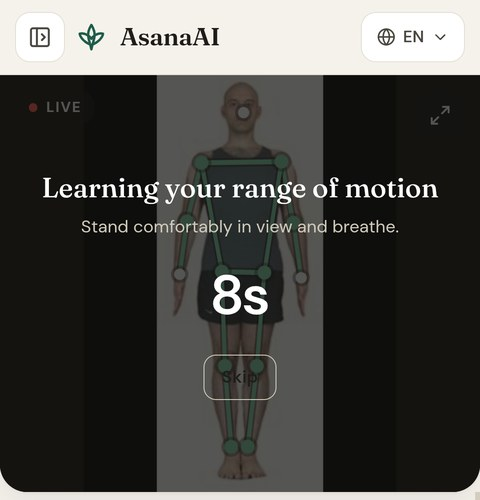
\includegraphics[width=\linewidth]{figures/cal_countdown.jpg}\caption{Calibration: 15\,s}\end{subfigure}\hfill
\begin{subfigure}[t]{0.19\textwidth}\centering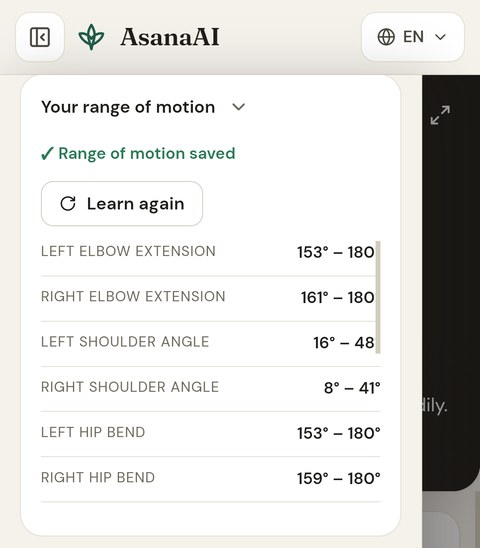
\includegraphics[width=\linewidth]{figures/cal_range.jpg}\caption{Saved range of motion}\end{subfigure}\hfill
\begin{subfigure}[t]{0.19\textwidth}\centering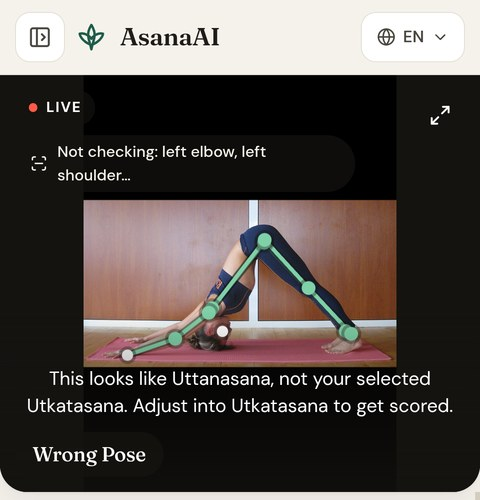
\includegraphics[width=\linewidth]{figures/fail_dog.jpg}\caption{Failure case}\end{subfigure}
\caption{(a)~Plank, guided mode: visible limbs are sage (inside their angle bands) and the chip ``Not checking: left elbow, left shoulder'' names joints the camera cannot see, which are drawn faint and neither scored nor coached. (b, c)~The personal profile: a 15\,s countdown and the saved per-joint ranges (the still photo yields narrow ranges). (d)~A failure shown on purpose: a Downward Dog photo is named Uttanasana (a forward fold), after which guided mode answers ``Wrong Pose''. Photos: Kennguru (a), Witold Fitz-Simon (b, c; CC BY-SA 2.5), Iveto (d); CC BY 3.0 unless noted, via Wikimedia Commons.}
\label{fig:proof}
\end{figure*}
